%%%%%%%%%%%%%%%%%%%%%%%%%%%%%%%%%%%%%%%%%%%%%%%%%%%%%%%%%%%%%%%%%%%%%%%%%%%%%%%%%%%%
% Document data
%%%%%%%%%%%%%%%%%%%%%%%%%%%%%%%%%%%%%%%%%%%%%%%%%%%%%%%%%%%%%%%%%%%%%%%%%%%%%%%%%%%%
\documentclass[12pt]{article} %report allows for chapters
%%%%%%%%%%%%%%%%%%%%%%%%%%%%%%%%%%%%%%%%%%%%%%%%%%%%%%%%%%%%%%%%%%%%%%%%%%%%%%%%%%%%
\usepackage{preamble}

\begin{document}

\begin{center}
   \textsc{\large MATH 271, Homework 0, \emph{Solutions}}\\
   \textsc{Due August 30$^\textrm{th}$}
\end{center}


\begin{problem}
    Compute the following:
\begin{enumerate}[(a)]
    \item $\displaystyle{\frac{d}{dx}(2x^7-3x^4+7)}$;
    \item $\displaystyle{\frac{d}{dt}\left(e^{at}\sin(bt)\right)}$;
    \item $\displaystyle{\frac{d}{ds}\left(\tan\left( e^{s^2}\right)\right)}$.
\end{enumerate}
\end{problem}

\begin{solution}~
\begin{enumerate}[(a)]
    \item Using the power, sum, and constant multiple rules we get
    \[
    \frac{d}{dx}\left( 2x^7 -3x^4 +y\right) = 14x^6-12x^3.
    \]
    \item Now using product and chain rule, we have
    \[
    \frac{d}{dt}\left( e^{at}\sin(bt)\right)= ae^{at}\sin(bt)+be^{at}\cos(bt).
    \]
    \item Using the chain rule twice, we have
    \[
    \frac{d}{ds} \left( \tan\left( e^{s^2}\right)\right) = \sec^2\left(e^{s^2}\right)2se^{s^2}.
    \]
\end{enumerate}
\end{solution}

\hrule

\begin{problem}
    Compute the following:
\begin{enumerate}[(a)]
    \item $\displaystyle{\int 2x^7-3x^4+7dx}$;
    \item $\displaystyle{\int_{-1}^1 \cos(t) dt}$;
    \item $\displaystyle{\int_0^1 e^{xy}dy}$;
\end{enumerate}
\end{problem}

\begin{solution}
~
\begin{enumerate}[(a)]
    \item Here, we use the power rule for antiderivatives to get
    \[
    \frac{1}{4} x^8 - \frac{3}{5} x^5 + 7x + c,
    \]
    where $c$ is an undetermined constant.
    \item Cosine is an \emph{even} function meaning that
    \[
    \cos(x)=\cos(-x).
    \]
    So we have
    \[
    \int_{-1}^1 \cos(t) dt = 2\int_0^1 \cos(t)dt.
    \]
    Then we use the fundamental theorem of calculus to get
    \[
    2\int_0^1 \cos(t)dt = 2 ( \sin(1)-\sin(0))=2\sin(1).
    \]
    \item Here, we need to make a substitution in that $z=xy$ so $dz=xdy$. Then we get
    \[
    \int_0^1 e^{xy}dy = \frac{1}{x} \int_0^xe^{z}dz.
    \]
    Then we can evaluate
    \[
    \frac{1}{x}\int_0^x e^z dz = \frac{1}{x}\left(e^x-1\right).
    \]
\end{enumerate}
\end{solution}

\hrule

\begin{problem}
    Find the point(s) of intersection of the parabola $f(x)=2x^2+2x+2$ and the line $g(x)=4x+4$ using algebra. Plot this on Desmos to confirm your answer and include a picture of the two graphs.
\end{problem}

\begin{solution}
Here's a picture of the two curves.
\begin{figure}[H]
    \centering
    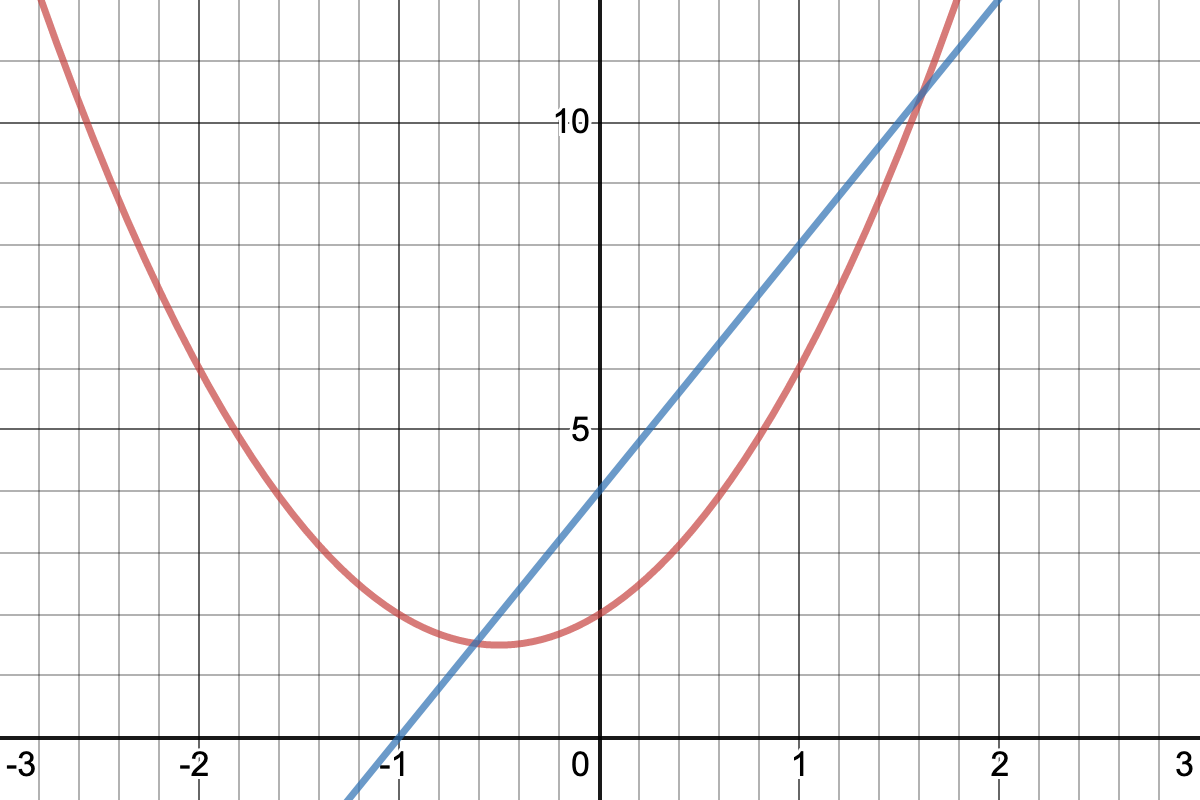
\includegraphics[width=.8\textwidth]{desmos-graph.png}
\end{figure}
We can see that they interesect in two points. We can find these intersections by setting the functions equal
\[
f(x)=g(x)
\]
which gives us
\begin{align*}
    2x^2+2x+2&=4x+4\\
    2x^2-2x-2&=0.
\end{align*}
So we can find the intersections by finding roots to a different (associated) polynomial. The roots (and thus intersections) are
\[
x=\frac{1}{2}\pm \frac{\sqrt{5}}{2}.
\]
\end{solution}

\hrule

\begin{problem}
    Now take the same parabola $f(x)=2x^2+2x+2$ and the line $h(x)=4x-4$. Plot this on Desmos and include a picture to show that the graphs of these two functions do not intersect in the plane. Explain why this must be true.
    
    We can find ``complex intersections" by doing the same algebra as the previous problem. Find these complex interesctions. (\emph{Hint: set up an equation whose roots would give you the intersections of these two curves.)}
\end{problem}

\hrule

\begin{solution}
Here's another picture.
\begin{figure}[H]
    \centering
    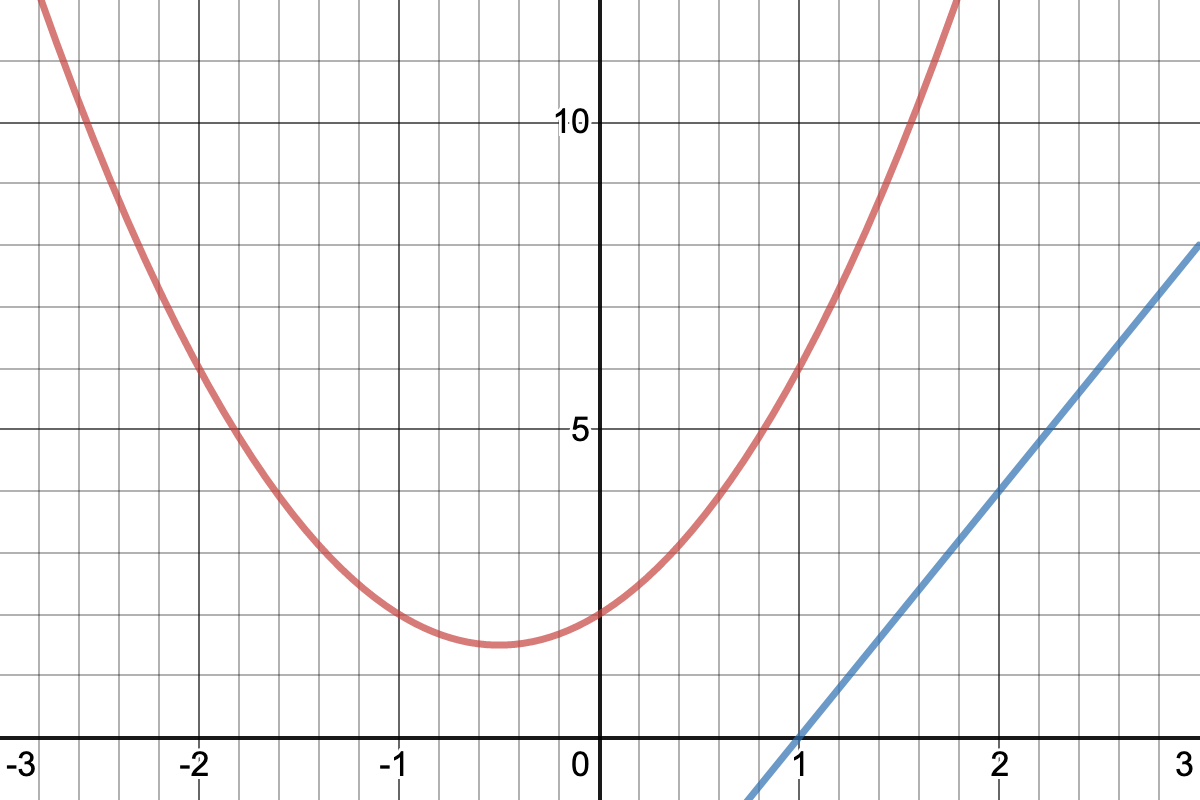
\includegraphics[width=.8\textwidth]{desmos-graph(2).png}
\end{figure}
Notice that these curves do not intersect when we allow only real number inputs. However, if we allow for complex inputs, then the functions can be equal. Algebraically, we have
\begin{align*}
    f(x)&=h(x)\\
    2x^2+2x+2&= 4x-4\\
    2x^2-2x+6&=0.
\end{align*}
The roots (or interesections) for this polynomial are then
\[
x=\frac{1}{2}\left( 1 \pm i \sqrt{11}\right).
\]
If you get used to complex numbers, you can wear your complex-goggles and see the interesection here! Honestly, I'm not great at wearing complex-goggles.
\end{solution}

\end{document}